\documentclass[11pt]{article}

\usepackage{fullpage}
\usepackage{amsmath}
\usepackage{booktabs}
\usepackage{makecell}
\usepackage{float}
\usepackage{graphicx}
\usepackage{pdfpages}
\usepackage{xcolor}
\usepackage[hidelinks]{hyperref}

\title{IE 58006 Heuristic Optimization\\Assignment 2: Tabu Search}
\author{Ulvi F\i nd\i k}
\date{\today}

\begin{document}

\maketitle

\begin{center}
Source code: \url{https://github.com/ulvifk/IE58006-Heuristic-HW2}
\end{center}

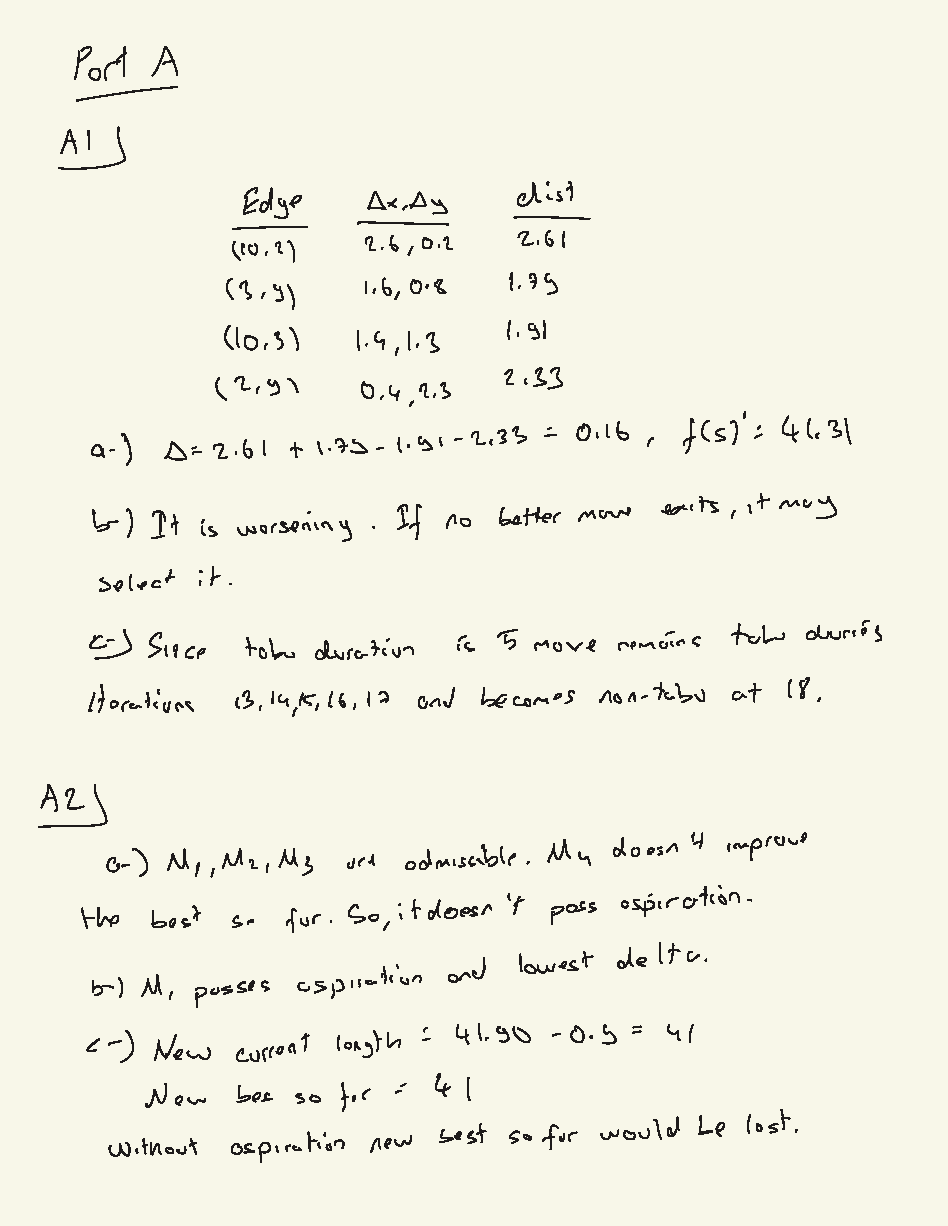
\includepdf[pages=1]{part_a_handwritten.pdf}

\section*{Part B: Implementation}

\subsection*{Implementation choices}

\begin{itemize}
    \item If two moves have the same score, the one with the smaller $i$ is selected, and if $i$ is also the same, the one with the smaller $j$. Here $i$ and $j$ are 0-based positions in the tour.
    \item Deltas and lengths are compared with a tolerance of $10^{-6}$. A tabu move passes aspiration, and a tour becomes the new best-so-far, only if it is shorter than the best-so-far by more than this tolerance.
    \item If every move is tabu and none passes aspiration, the run stops with an error. This does not happen in any of the runs.
\end{itemize}

\subsection*{B5: Baseline Run}

\begin{table}[H]
    \centering
    \begin{tabular}{ccccccccc}
\toprule
Iter. & $(i, j)$ & Removed & Inserted & $\Delta$ & Tabu & Aspiration & Current & Best \\
\midrule
1 & (13, 16) & (10,16) (11,17) & (10,11) (16,17) & -9.85 & no & yes & 84.30 & 84.30 \\
2 & (12, 19) & (18,10) (19,0) & (18,19) (10,0) & -9.03 & no & yes & 75.27 & 75.27 \\
3 & (10, 16) & (15,12) (16,13) & (15,16) (12,13) & -9.23 & no & yes & 66.04 & 66.04 \\
4 & (0, 3) & (0,4) (7,3) & (0,7) (4,3) & -6.44 & no & yes & 59.60 & 59.60 \\
5 & (6, 19) & (2,6) (10,0) & (2,10) (6,0) & -4.74 & no & yes & 54.86 & 54.86 \\
6 & (1, 19) & (7,1) (6,0) & (7,6) (1,0) & -3.66 & no & yes & 51.20 & 51.20 \\
7 & (10, 12) & (18,12) (13,11) & (18,13) (12,11) & -3.41 & no & yes & 47.79 & 47.79 \\
8 & (2, 18) & (6,8) (4,1) & (6,4) (8,1) & -1.72 & no & yes & 46.07 & 46.07 \\
9 & (2, 16) & (6,4) (15,5) & (6,15) (4,5) & -2.48 & no & yes & 43.59 & 43.59 \\
10 & (6, 9) & (14,19) (13,12) & (14,13) (19,12) & -1.53 & no & yes & 42.06 & 42.06 \\
11 & (13, 15) & (2,9) (3,4) & (2,3) (9,4) & -0.75 & no & yes & 41.31 & 41.31 \\
12 & (12, 14) & (10,2) (3,9) & (10,3) (2,9) & -0.16 & yes & yes & 41.15 & 41.15 \\
13 & (15, 17) & (9,4) (5,8) & (9,5) (4,8) & 0.88 & no & no & 42.03 & 41.15 \\
14 & (14, 17) & (2,9) (4,8) & (2,4) (9,8) & -0.36 & no & no & 41.67 & 41.15 \\
15 & (12, 14) & (10,3) (2,4) & (10,2) (3,4) & -0.85 & yes & yes & 40.82 & 40.82 \\
\bottomrule
\end{tabular}

    \caption{First 15 iterations of the baseline run ($d = 7$).}
    \label{tab:first-iterations}
\end{table}

\noindent\colorbox{gray!15}{\parbox{\dimexpr\linewidth-2\fboxsep}{
Final best tour:\\
$0 \to 1 \to 8 \to 9 \to 2 \to 3 \to 10 \to 11 \to 12 \to 13 \to 19 \to 18 \to 17 \to 14 \to 4 \to 5 \to 16 \to 15 \to 6 \to 7 \to 0$\\
Length: 40.57
}}


\begin{table}[H]
    \centering
    \begin{tabular}{ccc}
\toprule
Best & \makecell{Worsening\\moves} & \makecell{Aspiration\\uses} \\
\midrule
40.57 & 52 & 3 \\
\bottomrule
\end{tabular}

    \caption{Final best length, number of worsening moves selected and number of aspiration uses in the baseline run ($d = 7$, 100 iterations).}
    \label{tab:baseline-summary}
\end{table}

\begin{figure}[H]
    \centering
    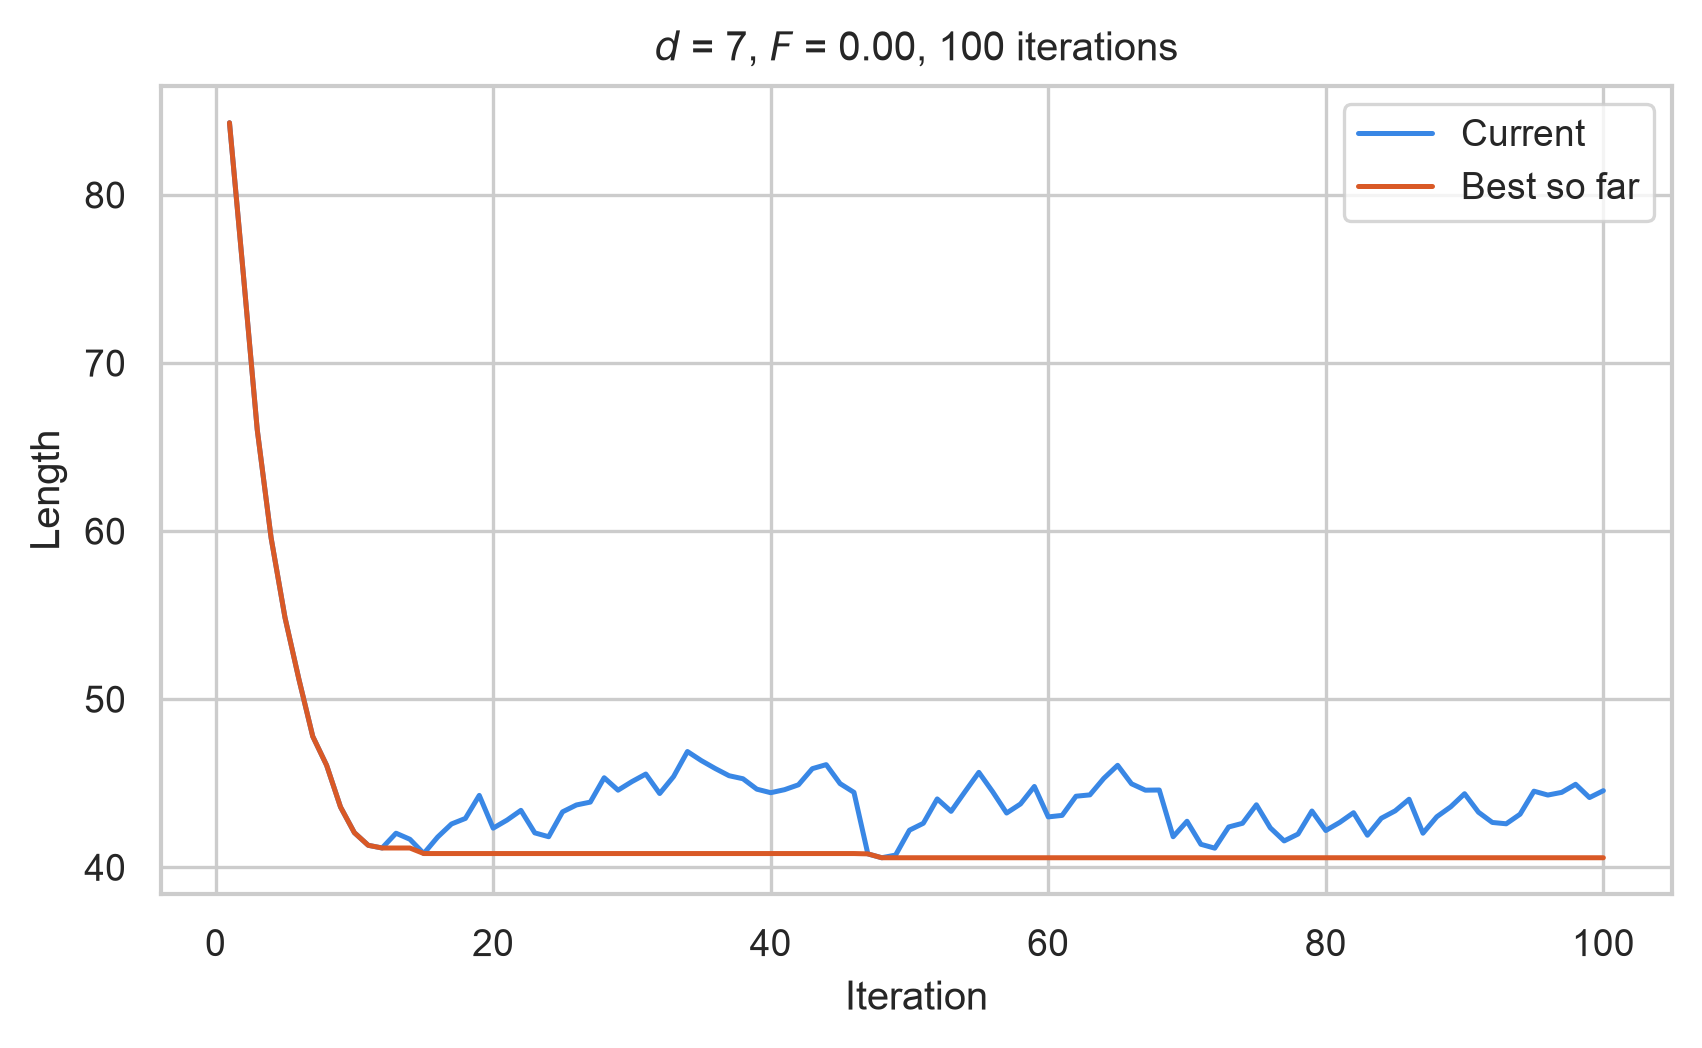
\includegraphics[width=\linewidth]{figures/length}
    \caption{Current and best-so-far tour length at each iteration of the baseline run ($d = 7$).}
    \label{fig:length}
\end{figure}

\begin{figure}[H]
    \centering
    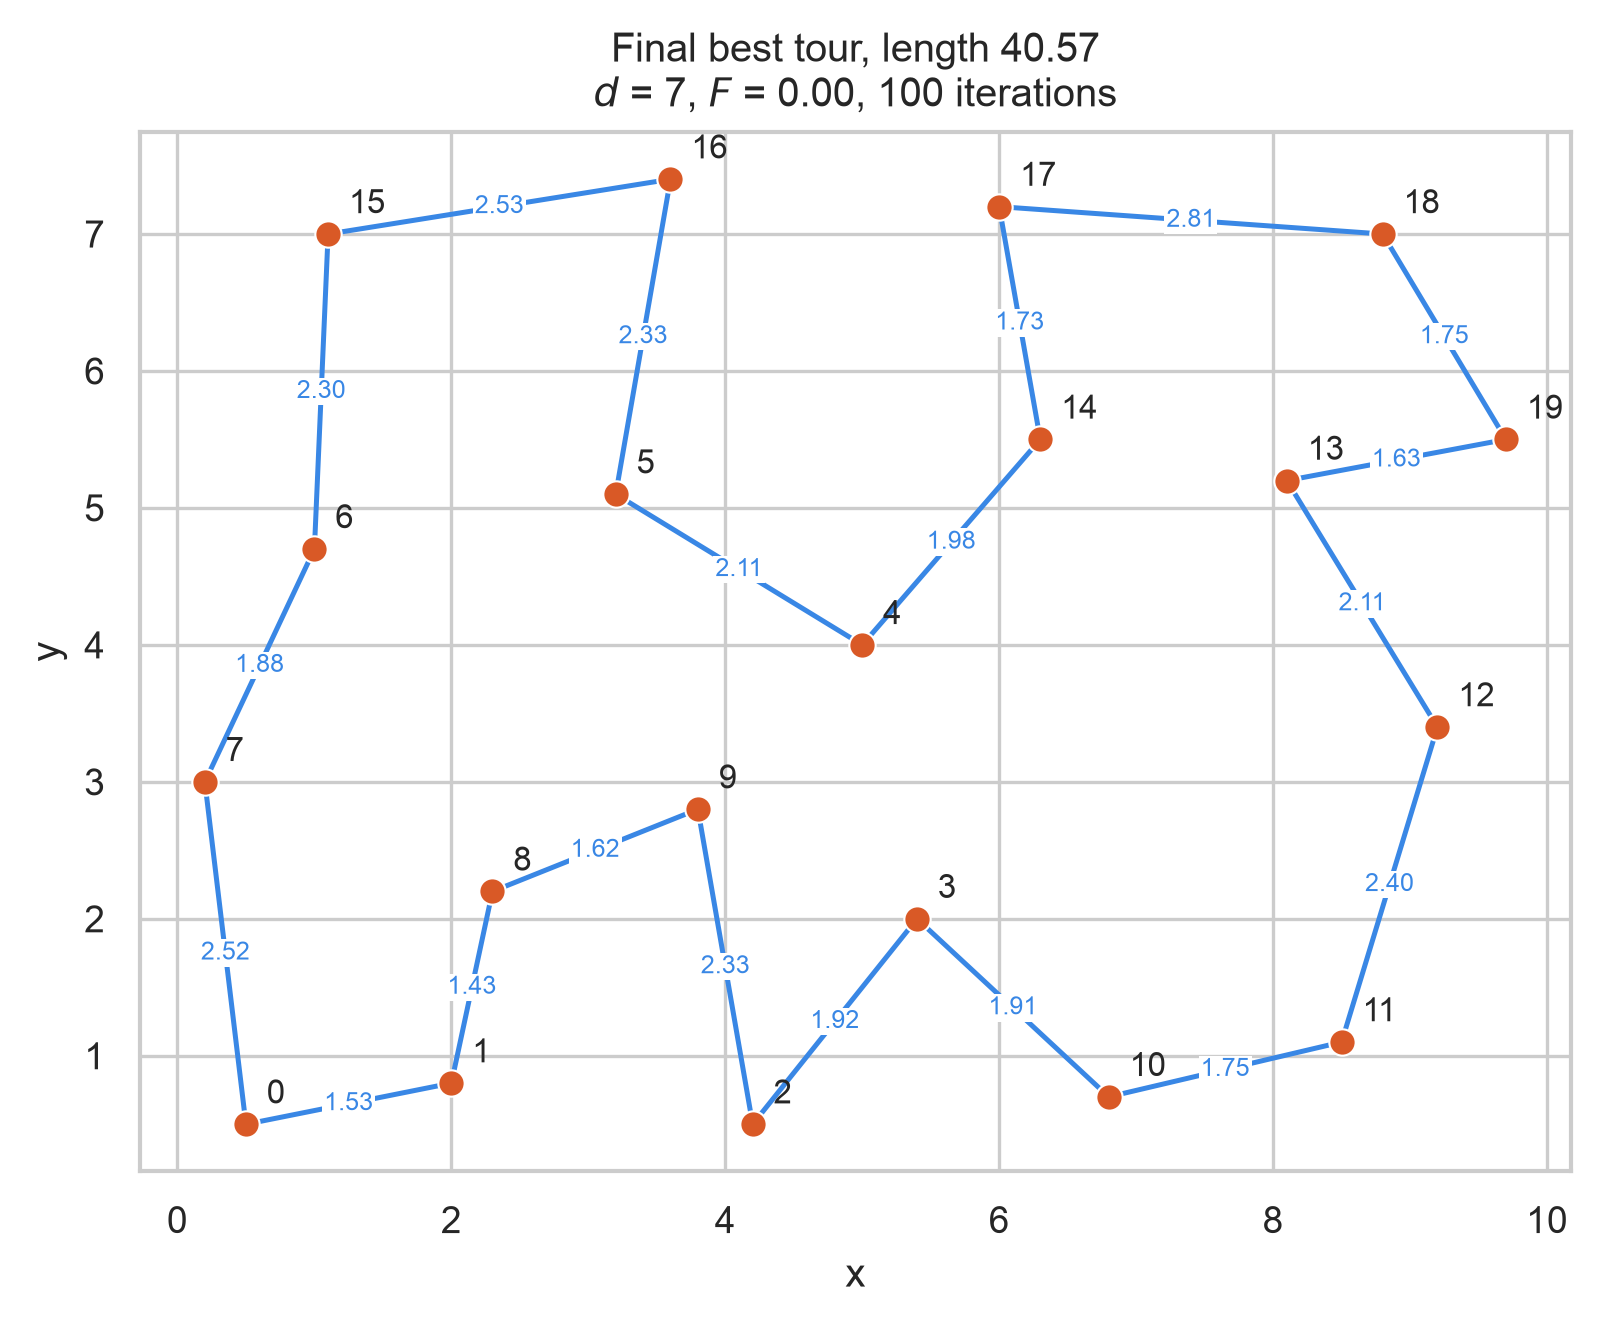
\includegraphics[width=\linewidth]{figures/final_best_tour}
    \caption{Final best tour of the baseline run ($d = 7$).}
    \label{fig:final-best-tour}
\end{figure}

\section*{Part C: Computational Experiments}

\subsection*{C1: Fixed Tabu Duration}

\begin{table}[H]
    \centering
    \begin{tabular}{ccccc}
\toprule
$d$ & Best & \makecell{Worsening\\moves} & \makecell{Aspiration\\uses} & \makecell{Repeated\\tours} \\
\midrule
0 & 41.15 & 44 & 0 & 88 \\
1 & 41.15 & 45 & 1 & 83 \\
3 & 40.57 & 37 & 2 & 61 \\
5 & 40.57 & 47 & 3 & 2 \\
7 & 40.57 & 52 & 3 & 0 \\
10 & 40.82 & 49 & 2 & 0 \\
15 & 40.82 & 49 & 2 & 0 \\
20 & 40.82 & 52 & 2 & 0 \\
\bottomrule
\end{tabular}

    \caption{C1: effect of the fixed tabu duration $d$ (100 iterations, no frequency penalty).}
    \label{tab:c1-fixed-tenure}
\end{table}

\begin{figure}[H]
    \centering
    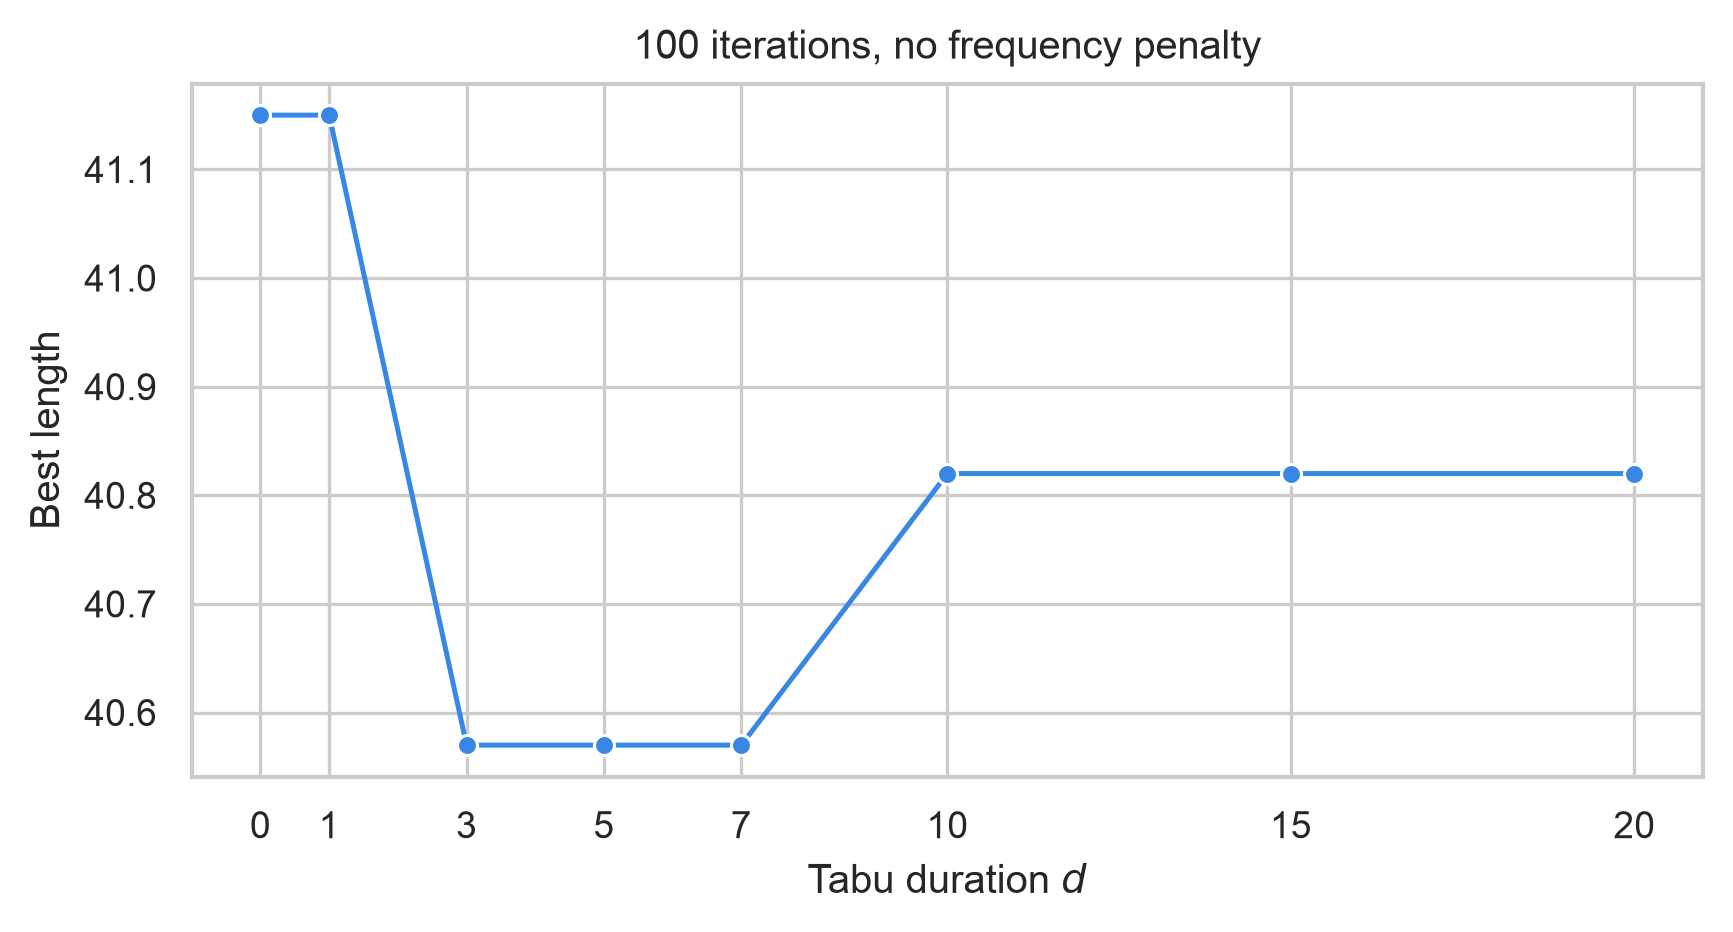
\includegraphics[width=\linewidth]{figures/c1_best_length}
    \caption{C1: final best length for each fixed tabu duration $d$.}
    \label{fig:c1-best-length}
\end{figure}

\paragraph{C1: trade-off.}
The best trade-off on this instance is around $d = 5$ to $7$. A shorter tenure lets the search cycle, and a longer one forbids useful moves. Table~\ref{tab:c1-fixed-tenure} and Figure~\ref{fig:c1-best-length} show both problems. With $d = 0$ and $d = 1$, the search reaches the local optimum of A1 (41.15) at iteration 12 and then cycles. With $d = 0$ it applies the A1 move ($\Delta = +0.16$) at iteration 13 and undoes it at iteration 14. It repeats these two tours for the rest of the run, so 88 of the 100 iterations revisit a tour. With $d = 1$ the cycle is only longer: four iterations (83 repeated visits). With $d = 3$ the search finds 40.57 at iteration 21, but then enters a cycle of ten iterations (61 repeated visits). From $d = 5$ on, the cycling stops: $d = 5$ revisits only 2 tours and $d \geq 7$ none. A long tenure causes the other problem. With $d \geq 10$ the search reaches 40.82 at iteration 15 and never improves on it, while $d = 5$ and $d = 7$ reach 40.57. Every removed edge stays forbidden for 10 or more of the 100 iterations, and some of the forbidden moves are the ones that lead to a shorter tour.

\subsection*{C2: Randomized Tabu Duration}

\begin{table}[H]
    \centering
    \begin{tabular}{cccc}
\toprule
$[d_{min}, d_{max}]$ & Best & Mean & Std. dev. \\
\midrule
$[2, 5]$ & 40.57 & 40.57 & 0.00 \\
$[5, 10]$ & 40.57 & 40.60 & 0.08 \\
$[7, 14]$ & 40.82 & 40.82 & 0.00 \\
$[10, 18]$ & 40.80 & 40.82 & 0.01 \\
\bottomrule
\end{tabular}

    \caption{C2: results when the tabu duration is drawn uniformly from $[d_{min}, d_{max}]$ at each selected move, over seeds 0--9 (100 iterations, no frequency penalty).}
    \label{tab:c2-random-tenure}
\end{table}

\paragraph{C2: comparison with fixed tenure.}
Randomizing the tenure mainly helps short tenures. Fixed $d = 3$ falls into a cycle with 61 repeated visits. With durations drawn from $[2, 5]$, the runs revisit only 9.5 tours on average. A cycle needs the same edges to be tabu at the same points again and again. When the durations vary, this does not happen. As Table~\ref{tab:c2-random-tenure} shows, the short ranges also give the best tours: $[2, 5]$ finds 40.57 on all ten seeds and $[5, 10]$ on eight of them. For long tenures, randomizing changes little. Their problem is too many forbidden moves, not cycling. $[7, 14]$ and $[10, 18]$ stop at 40.82, like the fixed tenures $d \geq 10$ (one seed of $[10, 18]$ reaches 40.80).

\subsection*{C3: Long-Term Frequency Memory}

\begin{table}[H]
    \centering
    \begin{tabular}{ccc}
\toprule
$F$ & Best & \makecell{Distinct\\tours} \\
\midrule
0.00 & 41.15 & 13 \\
0.05 & 40.82 & 23 \\
0.10 & 40.82 & 31 \\
0.20 & 40.57 & 50 \\
0.40 & 40.57 & 71 \\
\bottomrule
\end{tabular}

    \caption{C3: effect of the frequency penalty weight $F$ ($d = 0$, 100 iterations).}
    \label{tab:c3-frequency-penalty}
\end{table}

\paragraph{C3: interpretation.}
Frequency memory promotes diversification, but it makes up for $d = 0$ only partly. With $F = 0$ the run is the same as the $d = 0$ run of C1. It goes back and forth between the A1 local optimum and its neighbour and visits only 13 distinct tours. As Table~\ref{tab:c3-frequency-penalty} shows, a penalty on edges that were inserted often raises the number of distinct tours, up to 71 at $F = 0.40$. It also improves the best length, to 40.82 at $F = 0.05$ and $0.10$ and to 40.57 at $F = 0.20$ and $0.40$. This works because the two edges of the cycling move are inserted again and again. After a few times their penalty is larger than the small $\Delta$ of the cycle, so the search picks another move. At $F = 0.20$ and $0.40$ the search finds the same best length as the best fixed tenures. But it still revisits 51 and 30 tours, while $d = 7$ revisits none. At $F = 0.20$ the best tour appears only at iteration 95. The penalty stops a repeat only after it has happened several times. The tabu list forbids it at once.

\section*{Part D: Interpretation and Reflection}

\paragraph{(a)}
Short-term tabu memory remembers only the last few iterations and forbids moves. Long-term frequency memory remembers the whole run and only penalizes moves. The tabu list records which edges were removed recently. These edges cannot be inserted again for the next $d$ iterations, so the search cannot undo its last moves and cycle. After that, the edge is forgotten. Frequency memory counts how often each edge has been inserted over the whole run and never forgets. It forbids nothing. It adds $F \left[ c(a, c) + c(b, d) \right]$ to the score of a move. Moves that insert edges with high counts look worse, so the search tries edges it has used less.

\paragraph{(b)}
Iteration 13 of the baseline run (Table~\ref{tab:first-iterations}) selects a worsening move that leads to a later improvement. At iteration 12 the search reaches the 2-opt local optimum of A1, with length 41.15. No move improves it, so iteration 13 has to select a worsening move. The cheapest one is the A1 move with $\Delta = +0.16$. But it inserts $(10, 2)$ and $(3, 9)$ again, which iteration 12 removed, so it is tabu until iteration 19. The search selects the next best move instead, $(i, j) = (15, 17)$ with $\Delta = +0.88$, and the current length rises to 42.03. Then iteration 14 improves the tour to 41.67. Iteration 15 reaches a new best-so-far of 40.82, with a tabu move that aspiration allows.

\paragraph{(c)}
I recommend a tenure drawn from $[2, 5]$. In solution quality, it found 40.57 on all ten seeds, with a standard deviation of 0. This is the shortest tour any run found. In search behaviour, it reaches that tour at iteration 21.5 on average, so most of the 100 iterations are left as a margin. It also revisits only 9.5 tours on average, so it keeps visiting new tours instead of cycling like fixed $d = 3$. Fixed $d = 5$ also reaches 40.57 at iteration 21, with 2 repeated visits. But it is a single deterministic run, so it shows nothing about robustness. $[2, 5]$ shows the same quality over ten seeds.

\paragraph{(d)}
In tabu search, diversification comes from memory. In simulated annealing, it comes from randomness. Tabu search always takes the best allowed move, even if it makes the tour longer. At a local optimum no move improves the tour, so the search has to leave. The tabu list forbids the moves that would undo recent changes, so the search cannot fall back into the local optimum. Frequency memory also penalizes edges that were used often, so the search tries other edges. Simulated annealing draws a random move and accepts a worsening one with probability $e^{-\Delta / T}$. The temperature sets how often that happens.

\end{document}
